\documentclass{article}
\usepackage{listings}
\usepackage{minted2}
\usepackage{xcolor}
\usepackage{graphicx}
\usepackage{upquote}
\usepackage[left=2cm, right=2cm, top=2.5cm, bottom=2.5cm]{geometry}

\begin{document}

\title{LS26 : Agentic AI \\ \textbf{Week 1 Assignment}}
\author{Laxmi Bhargav Mende \\ 25B0940}

\maketitle
\tableofcontents
\newpage

\section{Question 1}
\subsection{Question}
Read the following scenario carefully.
“You are building a chatbot for a hospital. The chatbot needs to remember a
patient’s entire medical history (a 50 page document) while answering
follow up questions. You are using an LLM with a 4,000 token context
window.”\\
Why might this cause problems? What would happen if the medical history
exceeds the context window? Suggest one practical approach to handle this
limitation for the hospital chatbot.
\subsection{Answer}
Since it approximately take up 1 token per every 4 characters, a 4000 token context window only supports about 16,000 characters which is around 8-10 pages if formatted compactly.
The LLM here on trying to remenber te entire medical history will almost definitely hit the context window limit and in such a case they are generally designed such that the intial
content is forgotten or overwritten by the new data.\\
So as it tries to process the 50-page document it will remember only the end of the document and lack the beginning data.\\
A practical approach would be compress the history into a plain text removing any useless formatting or any kind of data which is unnessary or optional [i.e is sanitizing the input]


\newpage
\section{Question 2}
\subsection{Question}
 Write a Python script that uses the Anthropic API to do the
following. (You may refer to the Anthropic API documentation linked in the
resources).\\
Task: Build a simple ‘Study Buddy’ bot. The bot should:\\
\hspace*{15px}1. Accept a topic as an input from the user (e.g. “photosynthesis”)\\
\hspace*{15px}2. Send a request to the Claude API asking it to explain the topic in simple terms in under 100 words.\\
\hspace*{15px}3. Print the response to the terminal\\
\subsection{Answer}
\inputminted[breaklines, linenos, fontsize=\small]{python}{A1.py}
\begin{center}
	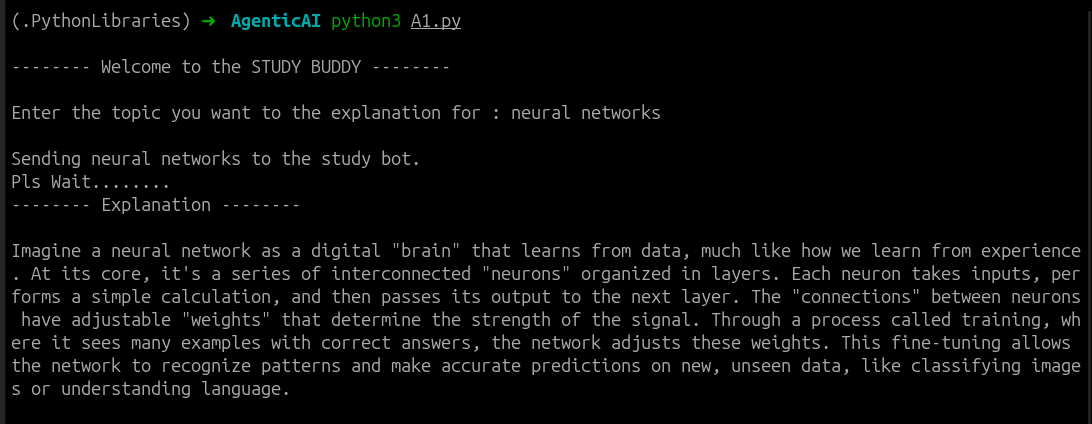
\includegraphics[scale=0.45]{runimg.png}
\end{center}
\newpage

\section{Question 3}
\subsection{Question}
Below is a task: classify the sentiment of a product review as
Positive, Negative, or Neutral.\\
“The delivery was on time but the product stopped working after two days.
Disappointed.”\\
\hspace*{15px}1. Write a zero-shot prompt for this task\\
\hspace*{15px}2. Write a few-shot prompt for the same task that includes at least 2
example review-label pairs before asking the model to classify the
given review.\\
\hspace*{15px}3. Which prompt do you expect to perform better for an LLM, and why?\\
\subsection{Answer}
\textbf{1. Zero-shot Prompt :}\\
\hspace*{15px}
Classify this product review as Positive, Neutral or Negative,\\
\hspace*{15px}
Review:"The delivery was on time but the product stopped working after two days. Disappointed.”
\\
\textbf{2. Few-Shot Prompt :}\\
\hspace*{15px}
Classify this product review as Positive, Neutral or Negative.\\
\hspace*{15px}
Here are sample classifications to use as a reference :\\
\hspace*{15px}
"Terrible customer service and the app crashes constantly." - Negative\\
\hspace*{15px}
"The battery life is incredible, easily lasting two full days of heavy use." - Positive\\
\hspace*{15px}
"Arrived scratched and missing the charger cord." - Negative\\
\hspace*{15px}
"Standard shipping took exactly as long as quoted." - Neutral\\
\hspace*{15px}
"Exceeded my expectations! The build quality is premium." - Positive\\
\hspace*{15px}
Review : "The delivery was on time but the product stopped working after two days. Disappointed."\\
\textbf{3. }The few-shot prompt is generally preferred as providing the LLM with a context helps it train itself to our requirements and here the format is similarl to finding the next probale word which the LLM is trained on, therby significantly improves it's effectiveness.
\\
\newpage

\section{Question 4}
\subsection{Question}
\textbf{Build a tool that will help IITB students plan their weekly study
schedule. A student provides:}\\
\hspace*{15pt}1. Their courses this semester (e.g. MA 110, CS 101, HS 101, etc.)\\
\hspace*{15pt}2. Number of hours available per day\\
\hspace*{15pt}3. Any upcoming exams or deadlines\\
\textbf{Complete the following tasks:}\\
\hspace*{15pt}1. Write a basic initial prompt for this task.\\
\hspace*{15pt}2. Identify two specific weaknesses or ambiguities in your initial prompt. Explain what could go wrong.\\
\hspace*{15pt}3. Write an improved prompt that fixes those weaknesses. Your improved prompt should specify: the output format (e.g. a table or a list), tone, and any constraints (like not scheduling more than 3 hours of one subject in a day).\\
\hspace*{15pt}4. Write a system prompt (1-3 sentences) you would give the model to set the right persona for this task.\\
\subsection{Answer}
\textbf{1. Basic Initial Prompt :}\\
\hspace*{15pt}Create a autonomous tool that will help IITB students plan their weekly study schedule. The student will provide their courses for that semester (e.g. MA 110, CS 101, HS 101, etc.), their number of hours available per day and any upcoming exams or deadlines. Make it such that it is easy-to-use and seamlessly integrates with their daily life.\\
\textbf{2. Weaknesses or Ambiguities :}
\begin{itemize}
\item\hspace*{15pt} It doesn't specify the type of architecture the tool needs to built upon, it can be a Web tool or an Android or an IOS tool.
\item\hspace*{15pt} The output form isnt specified, does it need to create a time-table or a checklist or any other form.
\item\hspace*{15pt} We donot specify the weightage of each course, some courses might require more time compared to others.
\item\hspace*{15pt} The meanong of seamlessly integrating is not specified properly and it might lead to various issues.
\item\hspace*{15pt} The persona or the mood of the tool is not mentioned, whether it should be formal or act as a companion or friend.
\end{itemize}
\textbf{3. Optimized Prompt :}
"Act as a senior software engineer. Write a complete, standalone Python script that generates an optimized weekly study schedule for an IIT Bombay student.\\
The script must prompt the user via the terminal for the following inputs:
\begin{itemize}
\item\hspace*{15pt} A list of their current semester courses, including the relative difficulty or credit weight (e.g., CS 101: 8 credits, HS 101: 6 credits).
\item\hspace*{15pt} Their fixed, unchangeable commitments (e.g., specific lecture times and lab hours).
\item\hspace*{15pt} The total number of free study hours they have available each day.
\item\hspace*{15pt} Any upcoming exam dates or project deadlines for the next 14 days.
\end{itemize}
The scheduling algorithm must adhere to these exact constraints:
\begin{itemize}
\item\hspace*{15pt} Prioritize study time for subjects with imminent deadlines or higher credit weights.
\item\hspace*{15pt} Implement spaced repetition by interleaving different subjects across the week rather than scheduling massive single-subject blocks.
\item\hspace*{15pt} Ensure no single study block exceeds 2 hours without a mandated 15-minute break.
\end{itemize}
Output Requirements:
\begin{itemize}
\item\hspace*{15pt} The script must print a clear, human-readable Markdown table of the schedule to the terminal.
\item\hspace*{15pt} The script must automatically generate and save a valid .ics (iCalendar) file containing the schedule, allowing the student to instantly import it into Google Calendar, Outlook, or Apple Calendar."
\end{itemize}
\textbf{4. System Prompt - Persona :}\\
\hspace*{15pt}You are a Senior Software Engineer and academic scheduling expert.
Convert complex constraints into functional Python code, prioritizing actionable outputs (e.g., .ics calendar files).

\end{document}
